% !TeX spellcheck = en_US
\addscenariosection{1}{Clash Scenario}{Arcane Artillery}{\images/berserk.png}

\begin{multicols}{2}

\textbf{Author:} NeuroN

\textbf{Source:} \href{https://discord.com/channels/740870068178649108/1279029213839626313}{Archon Studios Discord}

\textit{The ancient ruins are filled with arcane magic and technology, we must take control of them before our enemies can.
Some pieces of arcane artillery are scattered around the ruins, they can help us kill the dragons resting in them.}

\subsection*{\MakeUppercase{Scenario Length}}
This Scenario is played over 12 Rounds.

\subsection*{\MakeUppercase{Player Setup}}
\textbf{Player Count:} 2-6 Player FFA or 2vs2, 2vs2vs2, 3vs3 Alliance

\textbf{Starting Resources:} 10 \svg{gold}, 6 \svg{building_materials}, 1 \svg{valuables}

\textbf{Starting Income:} 15 \svg{gold}, 2 \svg{building_materials}, 1 \svg{valuables}

\textbf{Starting Units:}
\begin{itemize}
  \item a Few of each \svgunit{bronze} Unit
\end{itemize}

\textbf{Town Buildings:} \svgunit{bronze} Dwelling

\textbf{Map Tile Pool:} Each player takes 1 random Far (II--III) Map Tile, it must contain a Settlement

\subsection*{\MakeUppercase{Map Setup}}
Take the following Map Tiles and arrange them as shown in the Scenario map layout:

\textbf{For a 2-player Scenario:}
\begin{itemize}
  \item 2 × Starting (I) Map Tile
  \item 4 × Near (IV--V) Map Tile that contains an Obelisk. If not enough are available, treat Witch Huts as Obelisks
  \item 1 × Center (VI--VII) Map Tile, which must contain the Dragon Utopia Field
\end{itemize}

\textbf{For a 3-player Scenario:}
\begin{itemize}
  \item 3 × Starting (I) Map Tile
  \item 6 × Near (IV--V) Map Tile that contains an Obelisk. If not enough are available, treat Witch Huts as Obelisks
  \item 1 × Center (VI--VII) Map Tile, which must contain the Dragon Utopia Field
\end{itemize}

\textbf{For a 4-player Scenario:}
\begin{itemize}
  \item 4 × Starting (I) Map Tile
  \item 6 × Near (IV--V) Map Tile that contains an Obelisk. If not enough are available, treat Witch Huts as Obelisks
  \item 1 × Center (VI--VII) Map Tile, which must contain the Dragon Utopia Field
\end{itemize}

\textbf{For a 5-player Scenario:}
\begin{itemize}
  \item 5 × Starting (I) Map Tile
  \item 6 × Near (IV--V) Map Tile that contains an Obelisk. If not enough are available, treat Witch Huts as Obelisks
  \item 1 × Center (VI--VII) Map Tile, which must contain the Dragon Utopia Field
\end{itemize}

\textbf{For a 6-player Scenario:}
\begin{itemize}
  \item 6 × Starting (I) Map Tile
  \item 6 × Near (IV--V) Map Tile
  \item 1 × Center (VI--VII) Map Tile, which must contain the Dragon Utopia Field
\end{itemize}

\subsection*{\MakeUppercase{Victory Conditions}}
To win the Scenario, a Hero must Flag the Dragon Utopia Field.

\vspace*{\fill}

\subsection*{\MakeUppercase{Defeat Conditions}}
At the end of the \nth{12} Round, if there is no winner, all players lose the Scenario.

\subsection*{\MakeUppercase{Timed Events}}

\textbf{\nth{6} Round:}
\begin{itemize}
  \item Remove all Black cubes from every Tile.
\end{itemize}

\subsection*{\MakeUppercase{Additional Rules}}

Before the start of this Scenario:

\begin{itemize}
  \item If playing Alliance mode, allies and oppoents choose starting Tiles alternately.
\end{itemize}

During this Scenario:

\begin{itemize}
  \item Heroes cannot enter starting Tiles other than their own.
  \item A player may not use the Diplomacy card to skip Combat on the Dragon Utopia Field.
  \item Arcane Spikes are represented by cubes not used by any player's faction.
\end{itemize}

\vspace*{\fill}

\columnbreak

\begin{itemize}
    \item Obelisks may be captured. The first time an Obelisk is captured, gain one Arcane Spike.
    \item At the start of each player's turn, that player removes any unspent Arcane Spikes, then gains Arcane Spikes equal to the number of captured Obelisks they have.
\end{itemize}

\vspace{1em}

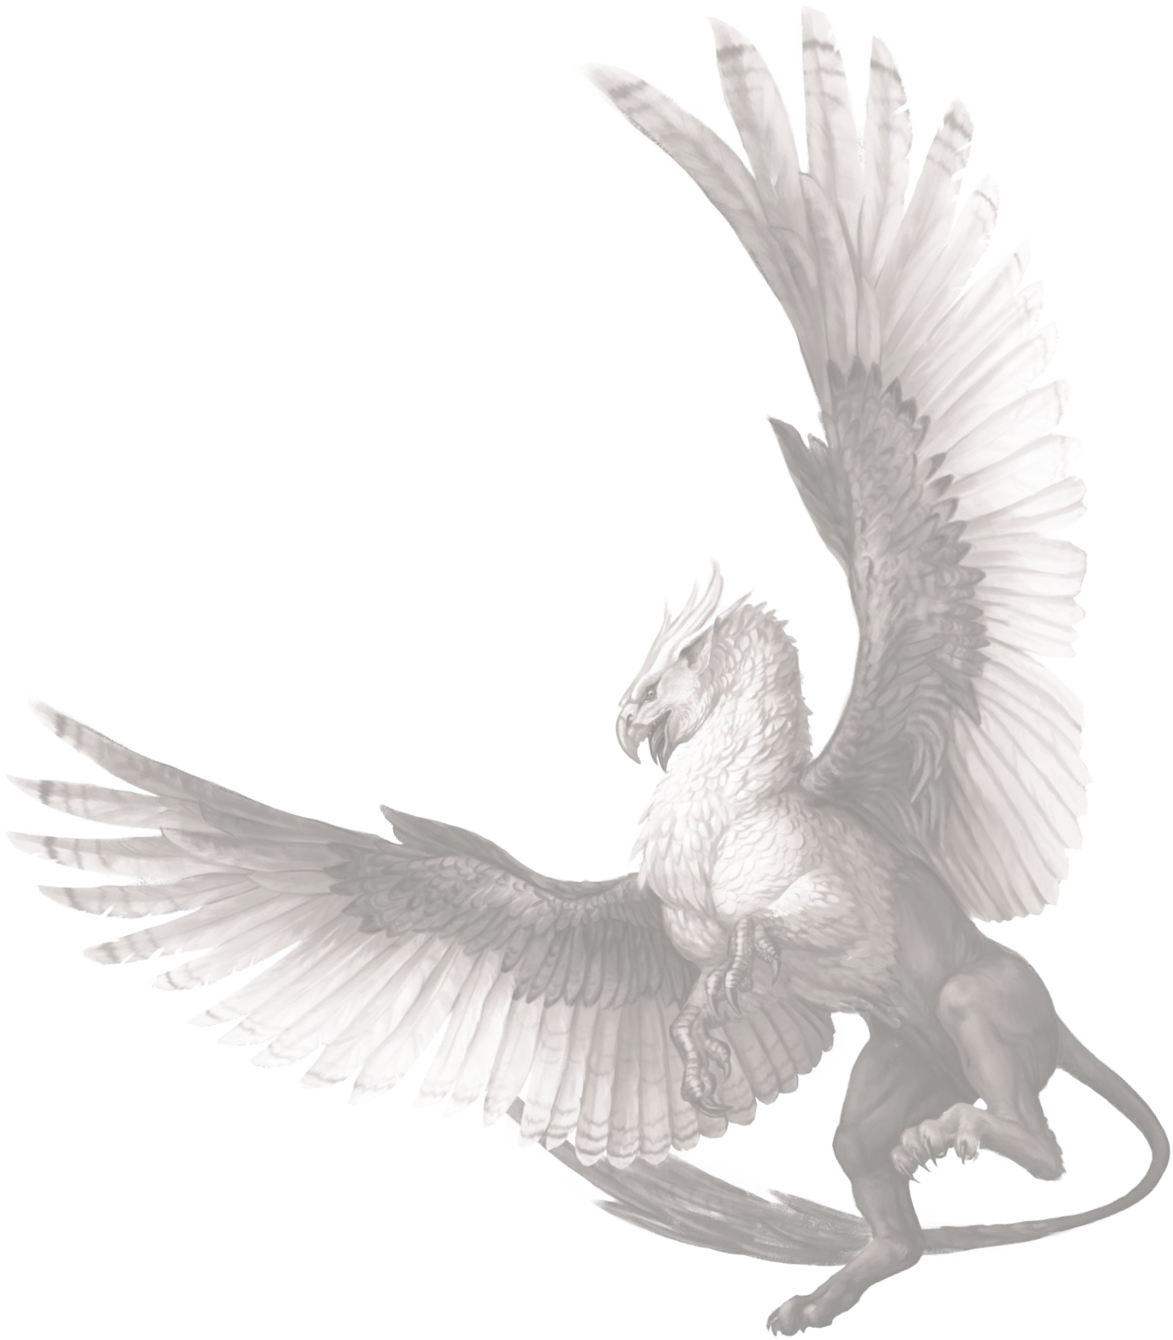
\includegraphics[width=\linewidth, keepaspectratio]{\art/griffin.png}

\end{multicols}

\vspace{1em}

\hommtable[]{15}{
  \begin{tabularx}{\linewidth}{X}
  \darkcell{\raisebox{-.2\height}{} \textbf{Activation Ability: Arcane Artillery}}\\
  \lightcell[4.8]{\raisebox{-.25\height}{} 
\includegraphics[height=10px]{\layout/listdot.png} Deal 1 \svg{damage-table} to target Unit by placing an Arcane Spike on it. \\ 
\includegraphics[height=10px]{\layout/listdot.png} Arcane artillery ignores the Azure Dragon's special ability. \\ 
\includegraphics[height=10px]{\layout/listdot.png} Arcane artillery does not count toward combat round spell limit. \\ 
\includegraphics[height=10px]{\layout/listdot.png} Arcane artillery is considered to be a spell of every school of magic. \\ 
\includegraphics[height=10px]{\layout/listdot.png} Players may cast Arcane Artillery when an opponent is in combat with neutral units, on the neutral units turn. \\ 
\includegraphics[height=10px]{\layout/listdot.png} Each player may only cast Arcane Artillery once per combat round. \\ 
\includegraphics[height=10px]{\layout/listdot.png} If playing Alliance mode, allies may cast Arcane Artillery on allied player's unit activation.} \\
  \end{tabularx}
}

\newpage

  \begin{minipage}{0.4\paperwidth}
    \centering
    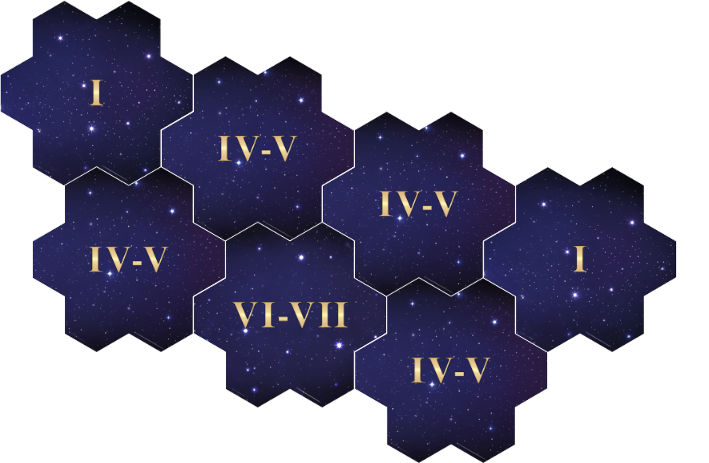
\includegraphics[width=0.36\paperwidth]{\maps/arcane_artillery_2p.png}
    \captionof{figure}{\textbf{2-PLAYER SCENARIO}}
  \end{minipage}
  \vspace{1em}
  \linebreak
  \begin{minipage}{0.4\paperwidth}
    \centering
    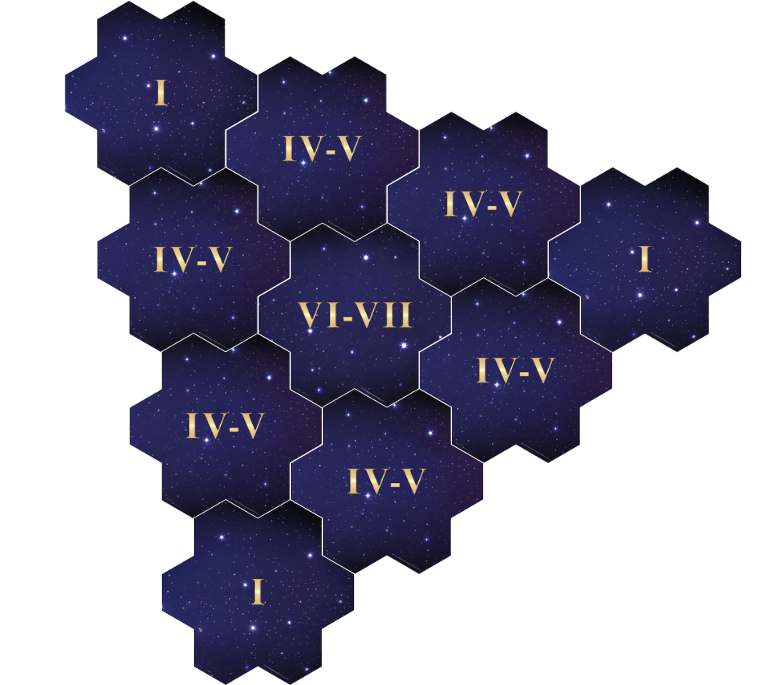
\includegraphics[width=0.38\paperwidth]{\maps/arcane_artillery_3p.png}
    \captionof{figure}{\textbf{3-PLAYER SCENARIO}}
  \end{minipage}
  \begin{minipage}{0.4\paperwidth}
    \centering
    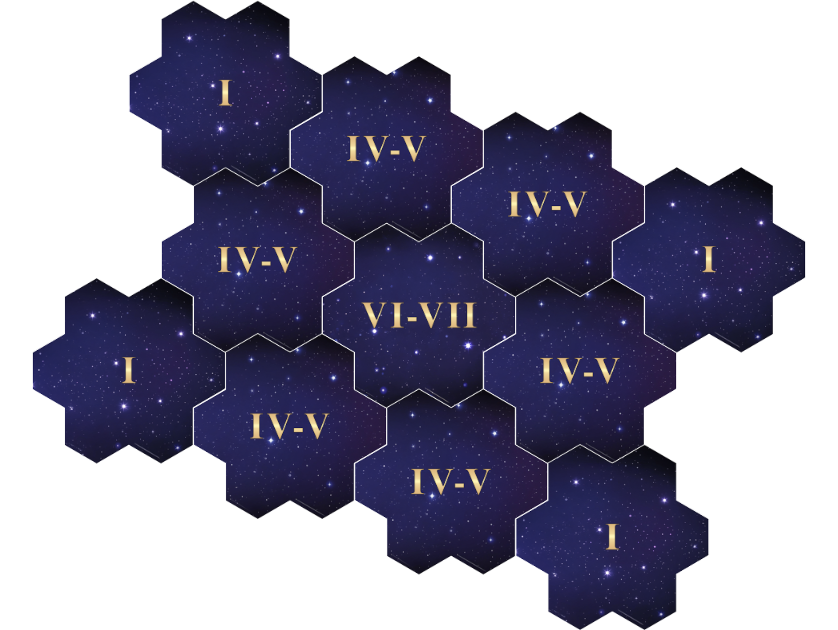
\includegraphics[width=0.38\paperwidth]{\maps/arcane_artillery_4p.png}
    \captionof{figure}{\textbf{4-PLAYER SCENARIO}}
  \end{minipage}
  \vspace{1em}
  \linebreak
  \begin{minipage}{0.4\paperwidth}
    \centering
    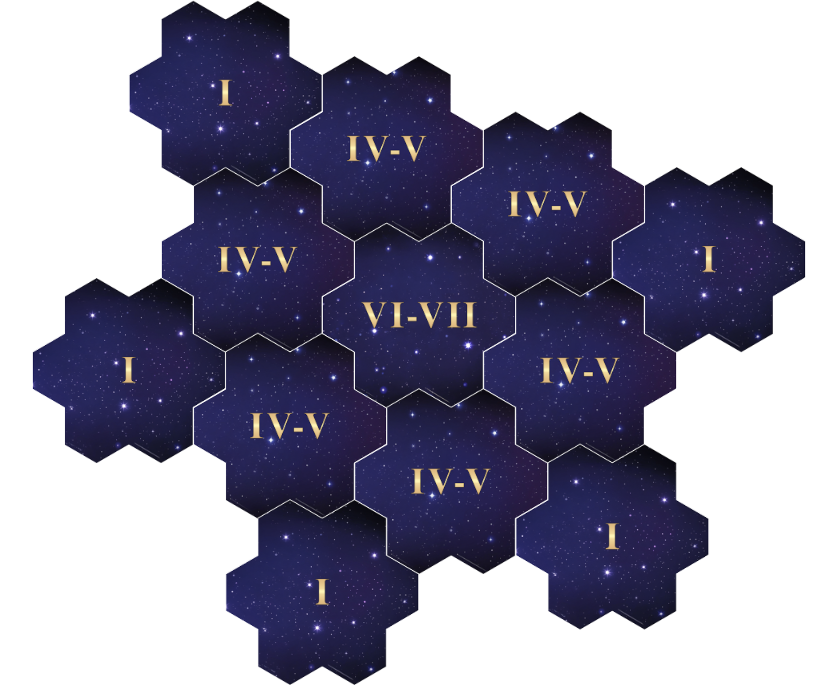
\includegraphics[width=0.38\paperwidth]{\maps/arcane_artillery_5p.png}
    \captionof{figure}{\textbf{5-PLAYER SCENARIO}}
  \end{minipage}
  \begin{minipage}{0.4\paperwidth}
    \centering
    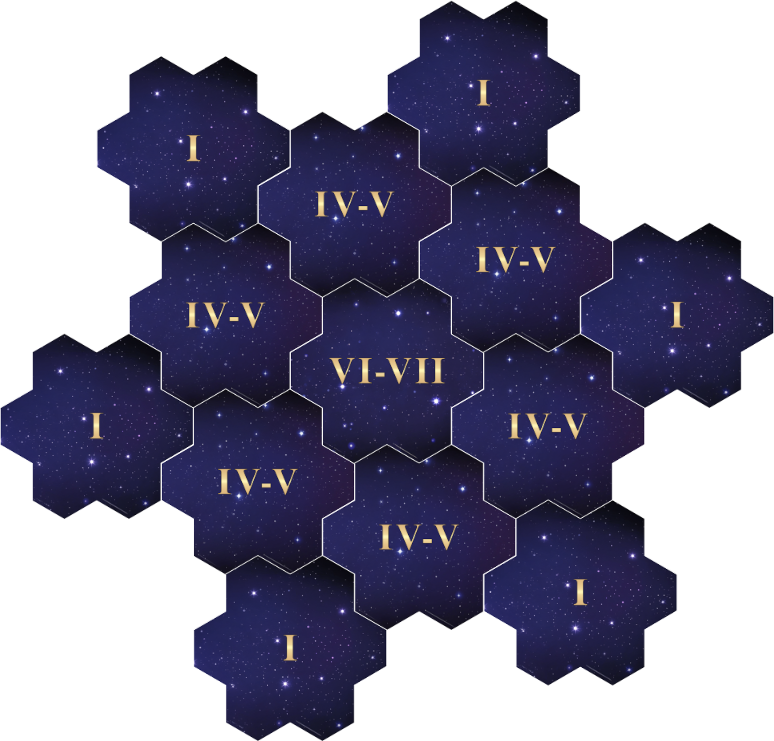
\includegraphics[width=0.38\paperwidth]{\maps/arcane_artillery_6p.png}
    \captionof{figure}{\textbf{6-PLAYER SCENARIO}}
  \end{minipage}
